\documentclass[tikz,border=10pt]{standalone}
\usepackage{tikz}
\usepackage{amsmath}
\usepackage{amssymb}
\usetikzlibrary{arrows.meta, calc, decorations.pathreplacing}

\begin{document}

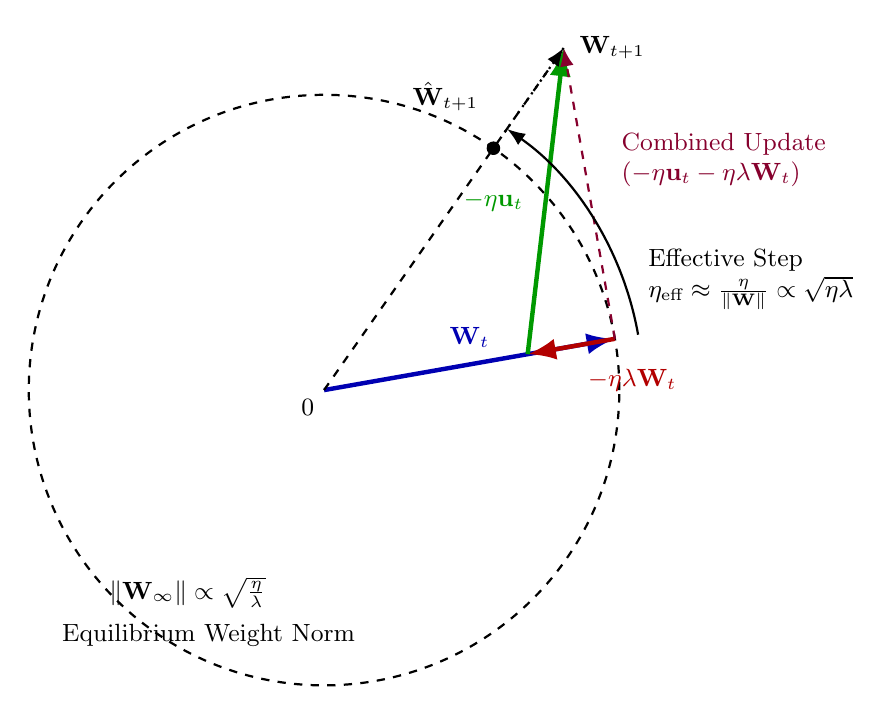
\begin{tikzpicture}[>=Latex, scale=1.5, font=\small]

    % --- 1. Define Coordinates ---
    % KEY: The COMBINED update (-η u_t - η λ W_t) is perpendicular to W_t,
    % NOT just the optimizer update alone. This shows weight decay's role
    % in constraining the weight norm to the equilibrium sphere.
    
    \coordinate (O) at (0,0); % Origin
    \def\R{2.5} % Radius of the sphere (equilibrium norm)
    \def\ang{10} % Angle of W_t (Modified to be more horizontal)

    % Extra radius for the effective-step arc
    \pgfmathsetmacro{\Rextra}{\R+0.2}

    % W_t coordinate
    \coordinate (Wt) at (\ang:\R);
    
    % Combined Update Vector (perpendicular to W_t)
    % Total update (-η u_t - η λ W_t) is perpendicular to W_t
    % Tangent direction is \ang + 90
    \coordinate (Wt_plus_1) at ($ (Wt) + ({\ang+90}:2.5) $);
    
    % Weight Decay Vector (pointing IN towards origin)
    % From W_t in the direction of -W_t (much smaller magnitude)
    \coordinate (Wt_decay_end) at ($ (Wt)!0.3!(O) $);

    % Projection of W_{t+1} back onto the sphere (Hat W_{t+1})
    % We calculate the angle of Wt_plus_1
    \pgfmathanglebetweenpoints{\pgfpointanchor{O}{center}}{\pgfpointanchor{Wt_plus_1}{center}}
    \let\angNew\pgfmathresult
    \coordinate (Wt_hat) at (\angNew:\R);

    % --- 2. Draw Axes and Sphere ---
    % Dotted circle for Equilibrium Norm
    \draw[dashed, thick] (O) circle (\R);
    
    % % Axes
    % \draw[->, thick, gray] (-3,0) -- (3,0);
    % \draw[->, thick, gray] (0,-3) -- (0,3);
    
    % --- 3. Main Vectors ---
    
    % W_t (Blue)
    \draw[->, ultra thick, blue!70!black] (O) -- (Wt) 
        node[midway, above, yshift=2pt, text=blue!70!black] {$\mathbf{W}_t$};
    
    % Weight Decay (Red) - From W_t pointing inward
    \draw[->, ultra thick, red!70!black] (Wt) -- (Wt_decay_end) 
        node[midway, below right, xshift=2pt, yshift=-4pt, align=left, text=red!70!black] {$-\eta \lambda \mathbf{W}_t$};

    % Optimizer Update (Green) - From decayed point to W_{t+1}
    \draw[->, ultra thick, green!60!black] (Wt_decay_end) -- (Wt_plus_1) 
        node[midway, above left, xshift=-4pt, yshift=-8pt, align=right, text=green!60!black] {$-\eta \mathbf{u}_t$};
    
    % Combined Update (Purple dashed) - From W_t to W_{t+1} to show total displacement
    \draw[->, thick, dashed, purple!70!black] (Wt) -- (Wt_plus_1) 
        node[midway, right, xshift=8pt, yshift=12pt, align=left, text=purple!70!black] {Combined Update\\$(-\eta \mathbf{u}_t - \eta \lambda \mathbf{W}_t)$};

    % W_{t+1} (Black dashed)
    \draw[->, thick, dashed] (O) -- (Wt_plus_1) 
        node[right, xshift=2pt] {$\mathbf{W}_{t+1}$};
    
    % --- 4. Projection / Effective Step ---
    
    % Effective Step arc between angles \ang and \angNew at radius \Rextra
    \draw[thick, ->] ({\ang}:\Rextra) arc (\ang:\angNew:\Rextra);
    \node[right, align=left] at ($ (Wt) + (0.2, 0.5) $) {Effective Step\\$\eta_{\text{eff}} \approx \frac{\eta}{\|\mathbf{W}\|} \propto \sqrt{\eta \lambda}$};

    % Mark the projected point \hat{W}_{t+1} on the circle
    \filldraw (Wt_hat) circle (1.5pt) node[anchor=south east, xshift=-2pt, yshift=10pt] {$\hat{\mathbf{W}}_{t+1}$};
    
    % Connection from W_{t+1} to \hat{W}_{t+1} (Projection)
    \draw[dotted, thick] (Wt_plus_1) -- (Wt_hat);

    % --- 5. Labels and Annotations ---
    
    % Equilibrium Label
    \node[anchor=north west] at (-\R+0.2, -\R+0.6) {Equilibrium Weight Norm};
    \node[anchor=north west] at (-\R+0.6, -\R+1) {$\|\mathbf{W}_\infty\| \propto \sqrt{\frac{\eta}{\lambda}}$};

    % Origin
    \node[below left] at (O) {$0$};

    % Orthogonality mark - circular arc showing 90° angle between W_t and combined update
    % Position arc on the right/exterior side
    % \draw[thick, purple!70!black] ($ (Wt) + ({\ang+90}:0.35) $) arc ({\ang+90}:{\ang+180}:0.35);
    % \node[purple!70!black, font=\scriptsize] at ($ (Wt) + ({\ang+135}:0.5) $) {$90^\circ$};

\end{tikzpicture}

\end{document}
